% Figure 3: (a) subtraction mean, (b) activation maps. Each PNG already holds both
% noOVS | OVS montages, the shared colorbar, the joint title and the white corner labels
% (../matlab/fig3_generate.m); this only stacks them and adds the panel letters.
% Build (from latex/): pdflatex -output-directory=../figures_assembled fig3.tex
\documentclass[tikz,border=2pt]{standalone}
\usepackage{graphicx}
\usepackage{helvet}
\renewcommand{\familydefault}{\sfdefault}

\def\W{17cm}     % width of each panel
\def\gy{0.3cm}   % gap between panels

\begin{document}
\begin{tikzpicture}
  \node[anchor=north west, inner sep=0] (a)
    {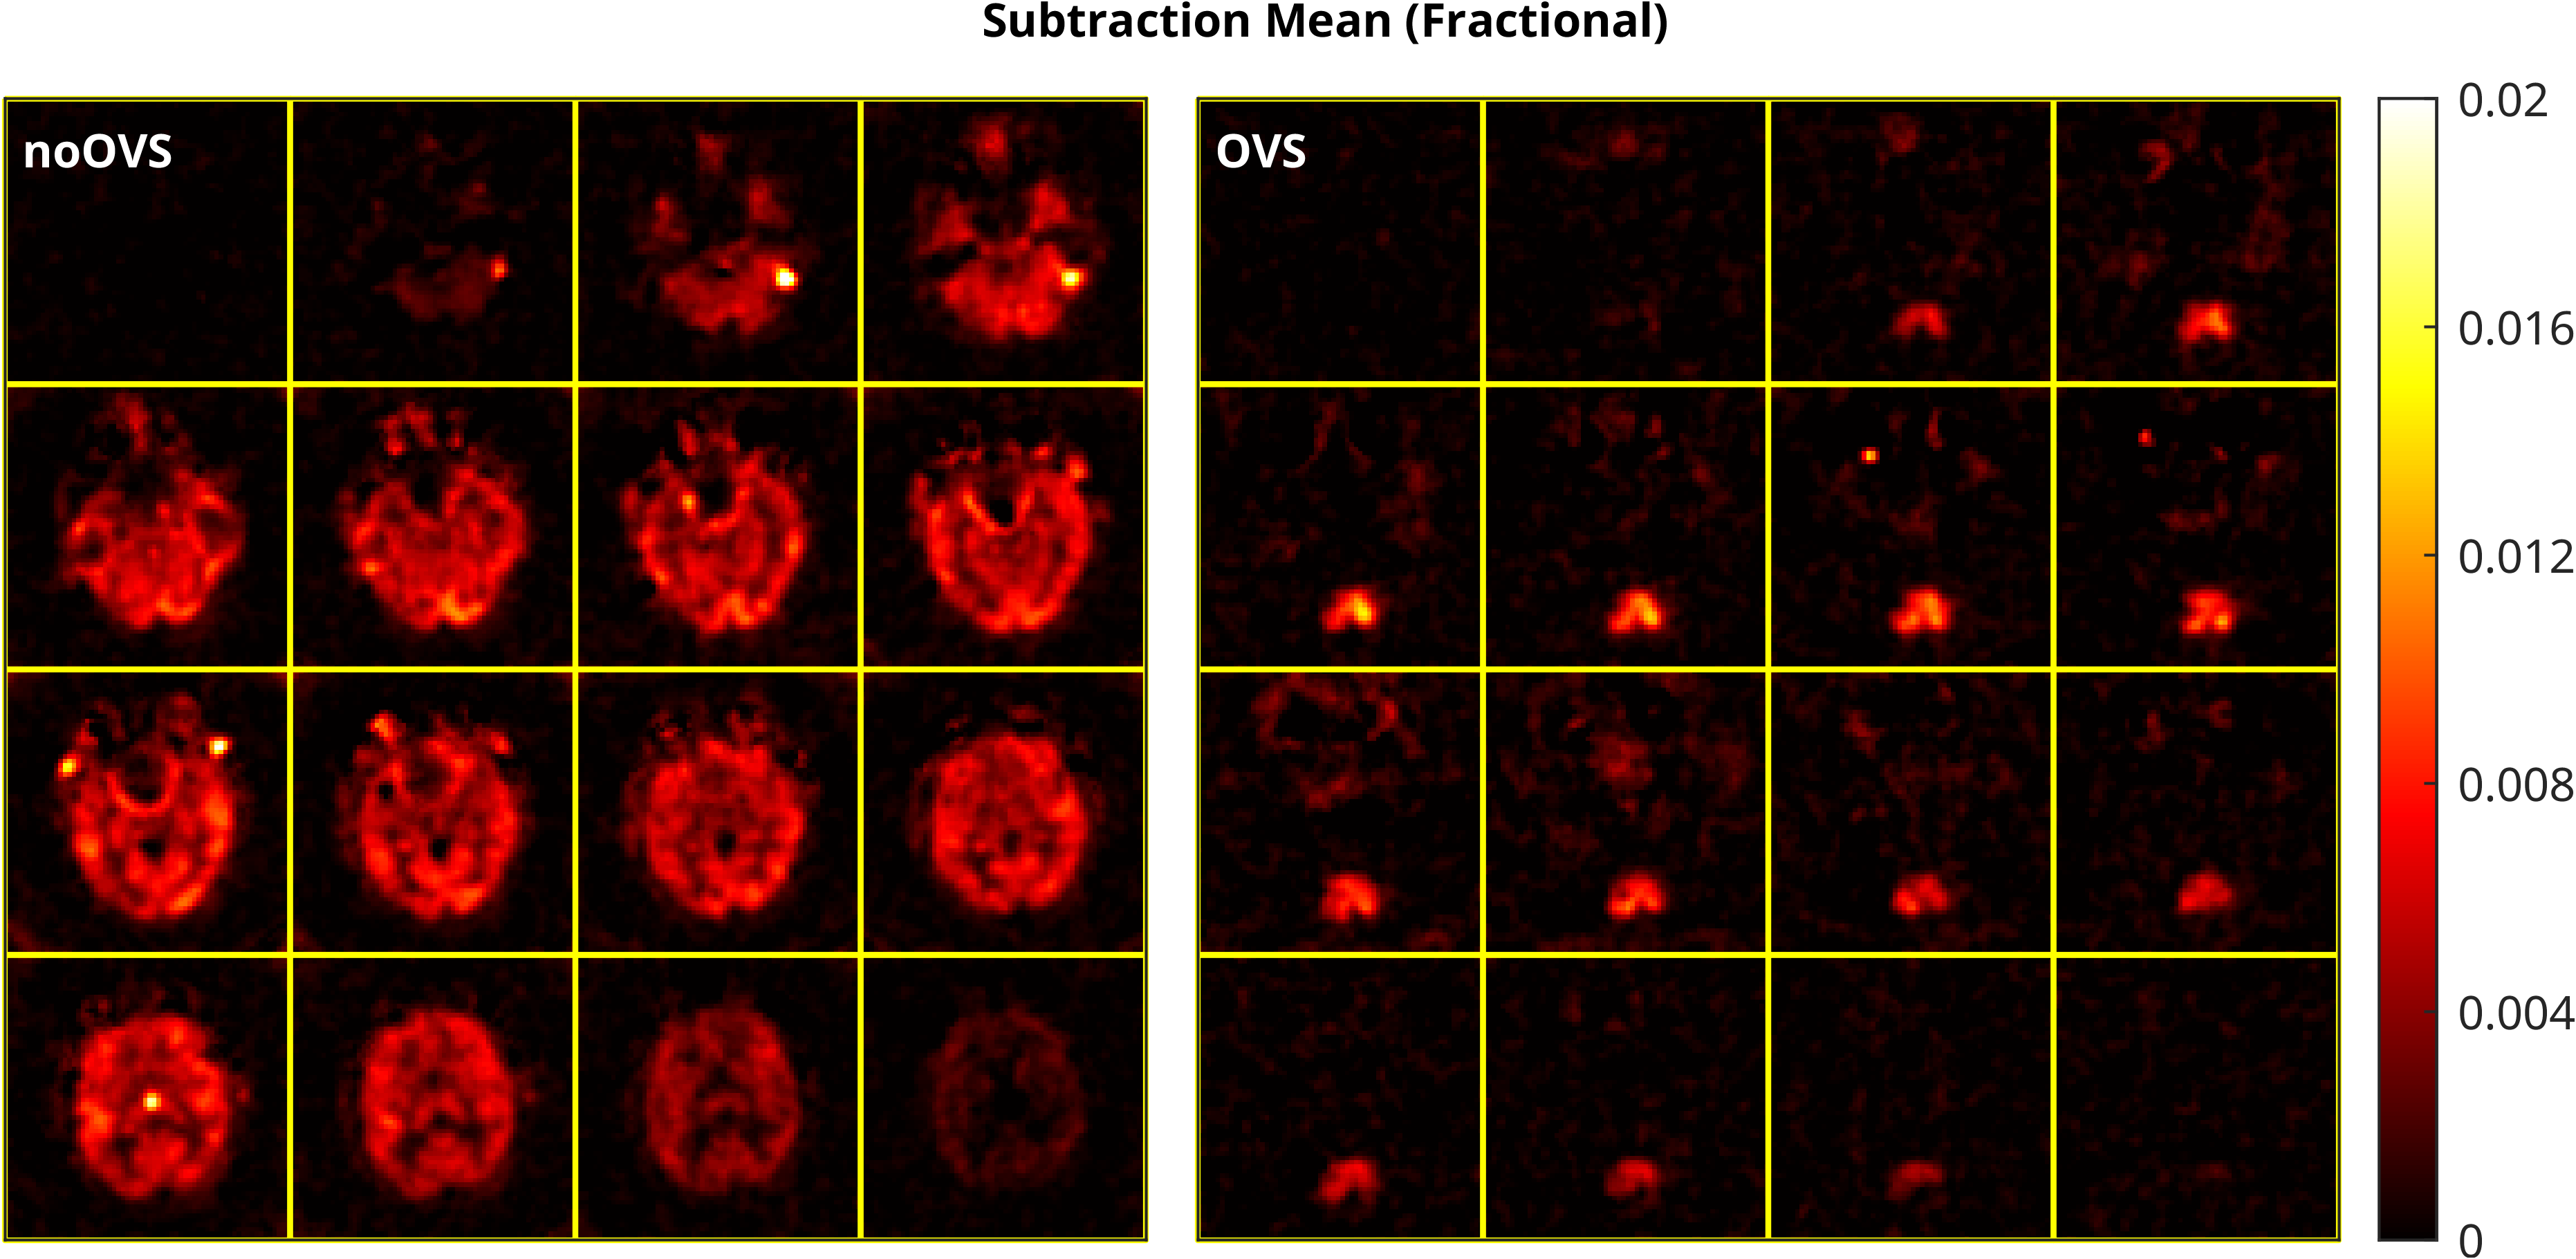
\includegraphics[width=\W]{../figures/fig3_subtraction_mean.png}};
  \node[anchor=north west, inner sep=0] (b) at ([yshift=-\gy]a.south west)
    {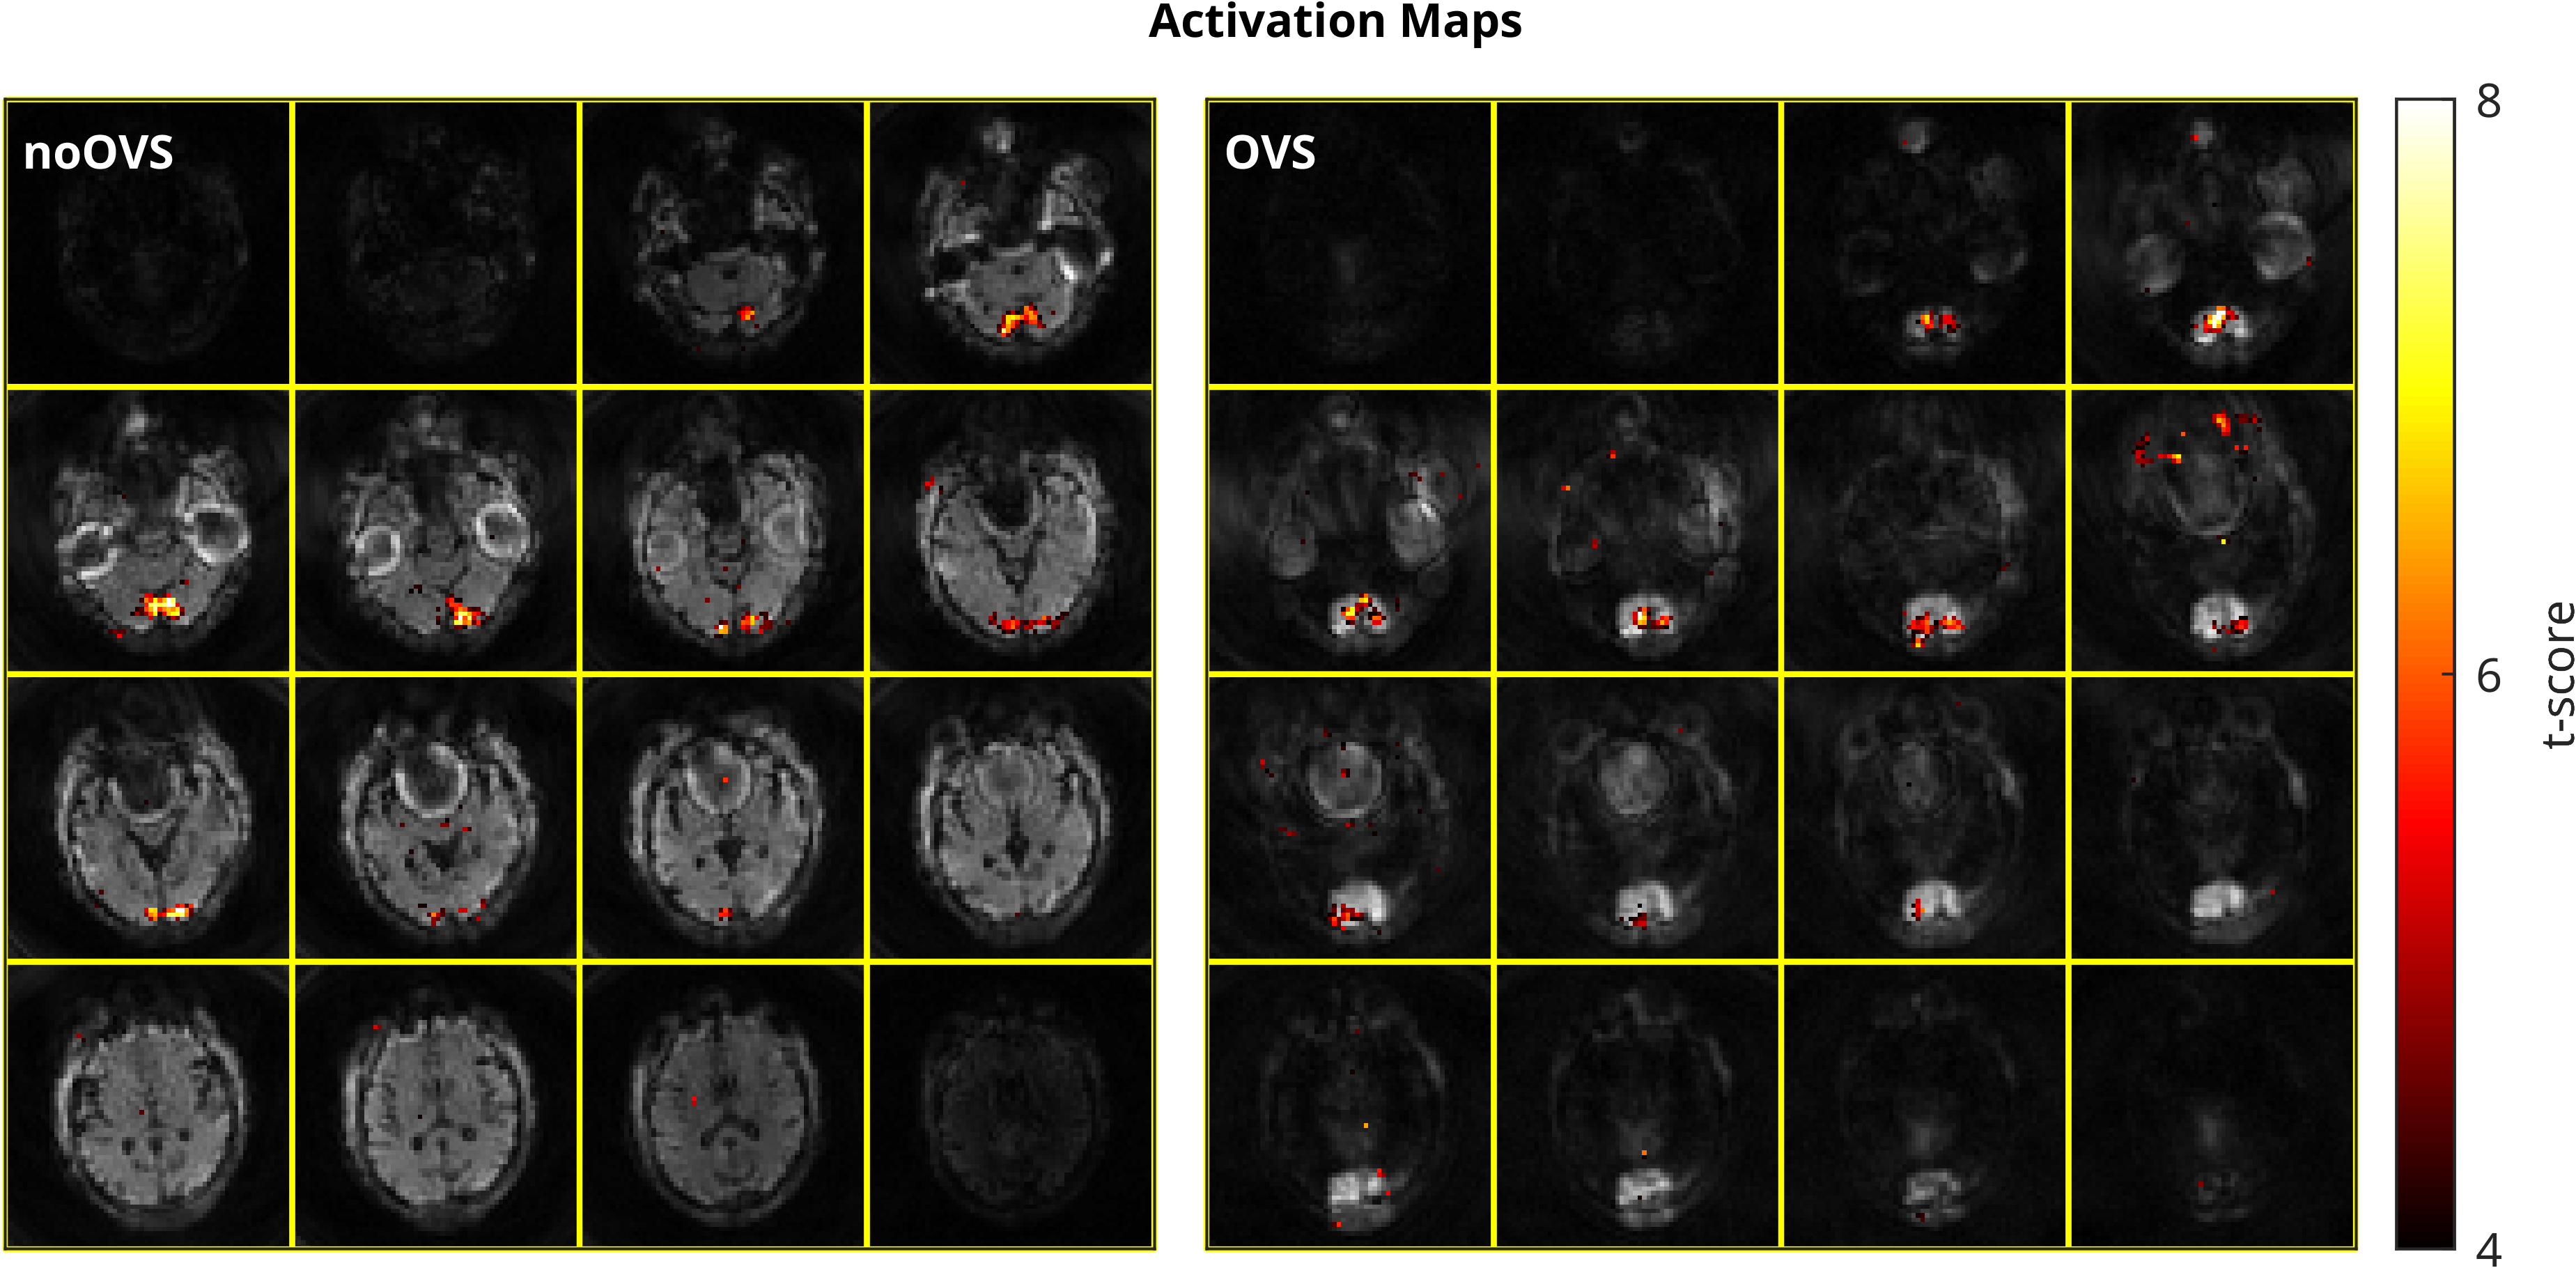
\includegraphics[width=\W]{../figures/fig3_overlay.png}};
  \foreach \n in {a,b}
    \node[anchor=north west, font=\bfseries, inner sep=0] at (\n.north west) {(\n)};
\end{tikzpicture}
\end{document}
